% GUID v6, Part III: every prediction other than rotation curves against current data. Numbers: docs/simulation/predictions_vs_data.py,
% results in docs/simulation/results/predictions_vs_data.{json,md}; \chk{data:Dn.m} names a row of that file.
\section{Every other prediction against current data}\label{sec:data}

The account of Part~I makes predictions well beyond galactic dynamics: universal free fall with an $\alpha$-setting scalar
(Sections~\ref{sec:fix} and~\ref{sec:alpha}), the post-Newtonian parameters of general relativity, a late universe that settles into
de Sitter expansion and a start that is inflation (Section~\ref{sec:cosmo}), Kerr black holes (Section~\ref{sec:bh}), the
Di\'osi--Penrose decoherence rate through Bridge~B (Section~\ref{sec:bridges}), primordial black holes as the contained remnant
(Section~\ref{sec:darkmatter}), and the electroweak and strong splits (Section~\ref{sec:matter}). This section confronts every one of
them that a published measurement reaches; rotation curves are treated in Sections~\ref{sec:sparc} and~\ref{sec:remnant} and are not
repeated. The result in one sentence: 54 of 58 scored confrontations are consistent with GUID at 95\%, the four that are not are
tensions GUID inherits unchanged from $\Lambda$CDM or from the plateau inflation Part~I names, and no datum yet reaches a prediction that
would tell GUID apart from general relativity, $\Lambda$CDM and the Standard Model \chk{data:summary}.

\subsection{Method}\label{sec:data-method}

Each confrontation sets a GUID value $x_G$, with a theory uncertainty $\sigma_G$ where one exists (for example propagated from Planck's
$\Omega_m$), against a datum. Data come in three forms. (i) A Gaussian measurement $x\pm\sigma$ at one standard deviation; we form the
\emph{pull}
\begin{equation}\label{eq:pull}
p=\frac{x-x_G}{\sqrt{\sigma^2+\sigma_G^2}} ,
\end{equation}
and a datum published as a 95\% interval of half-width $b$ enters with $\sigma=b/1.96$. (ii) An allowed region at a stated confidence level
of 90\% or more. (iii) A probability or a qualitative statement of the experimenters (the area theorem). The rule is one line: a
confrontation is \textbf{OK} when $|p|<z_{0.975}=1.96$, or when $x_G$ lies inside the allowed region; otherwise it is a \textbf{FAIL}, and it
stays a FAIL when general relativity, $\Lambda$CDM or the Standard Model share it. A 90\% region is narrower than the 95\% region of the
same measurement, so passing it implies passing at 95\%. A row is \textbf{INFO}, reported but not scored, when a newer measurement
supersedes it and includes its data, when it is derived rather than measured, or when it overlaps a scored datum; 14 of the 72 rows are
INFO. When independent determinations of one quantity disagree beyond their errors, we combine them with the weighted mean and the
scale factor of the Particle Data Group, $S=[\chi^2/(N-1)]^{1/2}$ with $S\ge1$, which multiplies the error of the mean. If GUID were right and
the 58 scored data were independent, about $0.05\times58=2.9$ FAILs would occur by chance; they are not all independent.

Every measured number was checked against its publication, mostly against the arXiv abstract or full text. Where the journal or
data-group pages could not be opened (the Particle Data Group, \emph{Nature}, ADS), the value was read through a web search of the
publication or of a review that quotes it; the results file lists, for each source, what was read and the value quoted. Six further checks
test the script's own numerics: a closed-form solution against its analytic limit, the Kerr efficiency at $a=-1,0,1$, and the
Di\'osi--Penrose self-energies against Fourier quadrature; all pass.

\subsection{Master table}\label{sec:data-table}

Table~\ref{tab:data-master} lists every scored confrontation, and Fig.~\ref{fig:data-pulls} shows the Gaussian pulls. Sources are
cited in the table; the subsections below explain each prediction and each test.

{\footnotesize\setlength{\tabcolsep}{3pt}
\begin{longtable}{@{}p{0.055\linewidth}p{0.28\linewidth}p{0.37\linewidth}p{0.17\linewidth}p{0.06\linewidth}@{}}
\caption{Every scored confrontation of GUID with data. Pull: Eq.~\eqref{eq:pull}, datum minus GUID; ``in'': the GUID value lies
inside the stated allowed region. Labels are the rows of \texttt{predictions\_vs\_data.json}.}\label{tab:data-master}\\
\toprule
ID & GUID prediction & Datum (1$\sigma$ unless stated) and source & Pull / test & Verdict \\
\midrule
\endfirsthead
\toprule
ID & GUID prediction & Datum and source & Pull / test & Verdict \\
\midrule
\endhead
\bottomrule
\endfoot
\multicolumn{5}{@{}l}{\emph{D1, the information scalar}}\\
D1.1 & free fall Ti/Pt: $\eta=2\lambda^2f_\oplus(f_{\rm Ti}-f_{\rm Pt})$, $0$ for the frame & $\eta=(-1.5\pm2.3\pm1.5)\times10^{-15}$ \cite{microscope} & $-0.55\sigma$ & OK\\
D1.2 & free fall Be/Ti & $\eta=(0.3\pm1.8)\times10^{-13}$ \cite{schlamminger2008} & $+0.17\sigma$ & OK\\
D1.3 & drift of $\alpha$ today, zero or negative & $(1.8\pm2.5)\times10^{-19}\,\mathrm{yr}^{-1}$ \cite{filzinger2023} & $+0.72\sigma$ & OK\\
D1.5 & $\Delta\alpha/\alpha$ 1.8\,Gyr ago & Oklo: $|\Delta\alpha/\alpha|<1.1\times10^{-8}$ (95\%) \cite{davis2015,damour1996} & in & OK\\
D1.6 & $\Delta\alpha/\alpha$ at $z=1.15$ & $(1.3\pm1.3\pm0.4)\times10^{-6}$ \cite{espresso} & $+0.96\sigma$ & OK\\
D1.7 & $\Delta\alpha/\alpha$ at $z=5.5$ to $7.1$ & $(-2.18\pm7.27)\times10^{-5}$ \cite{wilczynska2020} & $-0.30\sigma$ & OK\\
D1.8 & $\Delta\alpha/\alpha$ at recombination & $\alpha/\alpha_0=0.9993\pm0.0025$ \cite{hart2018} & $-0.28\sigma$ & OK\\
D1.9 & $\Delta\alpha/\alpha$ at nucleosynthesis & $(-7\pm5)\times10^{-3}$, $\alpha$ alone \cite{avelino2001} & $-1.40\sigma$ & OK\\
D1.12 & joint drift, Model B & $(1.79\pm2.49)\times10^{-19}\,\mathrm{yr}^{-1}$ (this work) & $+0.72\sigma$ & OK\\
\multicolumn{5}{@{}l}{\emph{D2, post-Newtonian gravity}}\\
D2.1 & $\gamma-1=0$ & Cassini: $(2.1\pm2.3)\times10^{-5}$ \cite{cassini} & $+0.91\sigma$ & OK\\
D2.2 & $\gamma-1=0$ & ephemerides: $(0.55\pm1.35)\times10^{-5}$ \cite{fienga2024} & $+0.41\sigma$ & OK\\
D2.3 & $\beta-1=0$ & ephemerides: $(-0.45\pm1.75)\times10^{-5}$ \cite{fienga2024} & $-0.26\sigma$ & OK\\
D2.4 & $\beta-1=0$ & MESSENGER: $(-1.6\pm1.8)\times10^{-5}$ \cite{genova2018} & $-0.89\sigma$ & OK\\
D2.5 & Nordtvedt $\eta_N=0$ & MESSENGER: $(-6.6\pm7.2)\times10^{-5}$ \cite{genova2018} & $-0.92\sigma$ & OK\\
D2.6 & $\beta-1=0$ & lunar laser ranging: $(6.2\pm7.2)\times10^{-5}$ \cite{biskupek2021} & $+0.86\sigma$ & OK\\
D2.7 & $\gamma-1=0$ & lunar laser ranging: $(1.7\pm1.6)\times10^{-4}$ \cite{biskupek2021} & $+1.06\sigma$ & OK\\
D2.8 & Earth--Moon $\Delta(m_g/m_i)=0$ & $(-2.1\pm2.4)\times10^{-14}$ \cite{biskupek2021} & $-0.88\sigma$ & OK\\
D2.9 & strong-field $\Delta=0$ & PSR J0337+1715: $(0.5\pm1.8)\times10^{-6}$ (95\%) \cite{voisin2020} & $+0.54\sigma$ & OK\\
D2.10 & redshift (lapse) as in GR & Galileo: $(0.19\pm2.48)\times10^{-5}$ \cite{delva2018} & $+0.08\sigma$ & OK\\
D2.11 & $c_{\rm gw}=c$ & $-3\times10^{-15}\le\Delta c/c\le7\times10^{-16}$ \cite{gw170817} & in & OK\\
D2.12 & graviton mass $0$ & $m_g\le2.42\times10^{-23}\,\mathrm{eV}/c^2$ (90\%) \cite{ligo2025a} & in & OK\\
\multicolumn{5}{@{}l}{\emph{D3, the balanced state}}\\
D3.1 & $z_t=0.632\pm0.018$ & $0.62\pm0.24$, two determinations, $S=3.2$ \cite{moresco2016,jesus2018} & $-0.06\sigma$ & OK\\
D3.3 & $w_0=-1$, $w_a=0$ & $\Lambda$CDM disfavoured at 2.8 to $4.2\sigma$ \cite{desi2} & $2.8\sigma$ (least) & \textbf{FAIL}\\
D3.4 & $H_0=67.4\pm0.5$ (CMB fit) & $73.04\pm1.04\,\mathrm{km\,s^{-1}Mpc^{-1}}$ \cite{riess2022} & $+4.89\sigma$ & \textbf{FAIL}\\
D3.5 & $H_0=67.4\pm0.5$ & $70.39\pm1.94$ (TRGB) \cite{freedman2025} & $+1.50\sigma$ & OK\\
D3.6 & $\Omega_K\approx0$ & flat to 0.4\% (95\%, with BAO) \cite{planck2020x} & in & OK\\
D3.7 & $\Omega_K\approx0$ & $(2.3\pm1.1)\times10^{-3}$ \cite{desi2} & $+2.09\sigma$ & \textbf{FAIL}\\
\multicolumn{5}{@{}l}{\emph{D4, inflation and the start}}\\
D4.1 & $n_s=1-2/N$, $N=50$ to 60 & $0.9649\pm0.0042$ \cite{planck2020x} & $+1.17$ to $-0.42\sigma$ & OK\\
D4.3 & $n_s=1-2/N$, $N=50$ to 60 & $0.974\pm0.003$ (P-ACT-LB) \cite{louis2025} & $+4.67$ to $+2.44\sigma$ & \textbf{FAIL}\\
D4.4 & $r=12/N^2=0.0033$ to $0.0048$ & $r<0.036$ (95\%) \cite{bk18} & in & OK\\
\multicolumn{5}{@{}l}{\emph{D5, black holes}}\\
D5.1 & thin-disk efficiency $\le0.423$ & $\epsilon=0.04$ to $0.16$ \cite{marconi2004} & in & OK\\
D5.2 & same & $\epsilon=0.075$ to $0.094$ \cite{shankar2009} & in & OK\\
D5.3 & same & $\epsilon>0.1$ for luminous quasars \cite{yu2002} & in & OK\\
D5.4 & same & mean $\epsilon=0.089$ \cite{davis2011} & in & OK\\
D5.5 & Kerr bound $|a|\le1$ & 61 spins, 90\% ranges \cite{reynolds2021} & 0 outside & OK\\
D5.6 & area never shrinks & GW150914: $P(\Delta A>0)=0.97$ \cite{isi2021} & agrees & OK\\
D5.7 & area never shrinks & GW250114: ``to high credibility'' \cite{ligo2025b} & agrees & OK\\
\multicolumn{5}{@{}l}{\emph{D6, Bridge B (Di\'osi--Penrose rate)}}\\
D6.1 & $\Gamma\tau\ll1$ & 28\,kDa molecules, 266\,nm, about 7\,ms \cite{fein2019} & $\Gamma\tau=6\times10^{-15}$ & OK\\
D6.2 & $\Gamma\tau\ll1$ & 197\,kDa Na clusters, ${\ge}80$\,nm, 12\,ms \cite{pedalino2025} & $\Gamma\tau=2\times10^{-13}$ & OK\\
D6.3 & $\Gamma\tau\ll1$ & Rb atoms, 54\,cm, 1\,s \cite{kovachy2015} & $\Gamma\tau=2\times10^{-16}$ & OK\\
D6.4 & $\Gamma\tau\ll1$ & Cs atoms, 3.9\,$\mu$m, 20\,s \cite{xu2019} & $\Gamma\tau=1\times10^{-14}$ & OK\\
D6.5 & $R_0\ge4\times10^{-10}$\,m & $R_0>0.54\times10^{-10}$\,m (95\%) \cite{donadi} & in & OK\\
D6.6 & same & $R_0\gtrsim4\times10^{-10}$\,m \cite{figurato} & in & OK\\
D6.7 & same & $R_0\ge4.0\times10^{-14}$\,m, detector heating, as quoted in \cite{donadi} & in & OK\\
D6.8 & $l_P^2D_2=m_P^2/c=1.6\times10^{-24}$\,kg$^2$\,s/m & window $10^{-40}$ to $10^{-9}$ \cite{osswd} & in & OK\\
\multicolumn{5}{@{}l}{\emph{D7, contained remnants}}\\
D7.1 & PBHs of $10^{17}$ to $10^{22}$\,g can be all dark matter & window open \cite{gortongreen} & agrees & OK\\
D7.2 & evaporated below $1.7\times10^{11}$\,kg & about $10^{15}$\,g \cite{carr2021} & within $\times10$ & OK\\
\multicolumn{5}{@{}l}{\emph{D8, the electroweak and strong splits}}\\
D8.1 & proton decay possible, $\tau\sim5\times10^{35}$\,yr & $\tau/B(p\to e^+\pi^0)>2.4\times10^{34}$\,yr (90\%) \cite{superk} & in & OK\\
D8.2 & no relic monopoles & flux $<1.4\times10^{-16}\,\mathrm{cm^{-2}s^{-1}sr^{-1}}$ (90\%) \cite{macro} & in & OK\\
D8.3 & $m_W=gv/2=80.22$\,GeV, within 0.5\% & $80.369\pm0.013$\,GeV \cite{lhctev2024} & $-0.18\%$ & OK\\
D8.4 & $m_Z=m_W/\cos\theta_W=91.50$\,GeV & $91.1880\pm0.0020$\,GeV \cite{navas2024} & $+0.34\%$ & OK\\
D8.5 & $1/\alpha\approx128$ at the split & $1/\hat\alpha(M_Z)=127.950\pm0.017$ \cite{erler2017} & within 1\% & OK\\
D8.6 & split is a crossover & $m_H=125.11\pm0.11$\,GeV $>95$\,GeV \cite{atlas2023,kajantie1996} & in & OK\\
\multicolumn{5}{@{}l}{\emph{D9, the rest}}\\
D9.1 & CHSH $S\le2\sqrt2$, attained & $S=2.82759\pm0.00051$ \cite{poh2015} & $-1.64\sigma$ & OK\\
D9.2 & $2<S\le2\sqrt2$ & loophole-free $S=2.42\pm0.20$ \cite{hensen2015} & in & OK\\
D9.3 & neutrinos are not the remnant & $\sum m_\nu<0.064$\,eV: below 0.57\% of $\Omega_c$ \cite{desi2} & in & OK\\
D9.4 & same & $m_\nu<0.45$\,eV (90\%): below 12\% \cite{katrin2025} & in & OK\\
D9.5 & GW background is not dark matter & $\Omega_{\rm gw}\le1.3\times10^{-8}$ at 1/yr \cite{nanograv} & in & OK\\
\end{longtable}}

\begin{figure}[tbp]
\centering
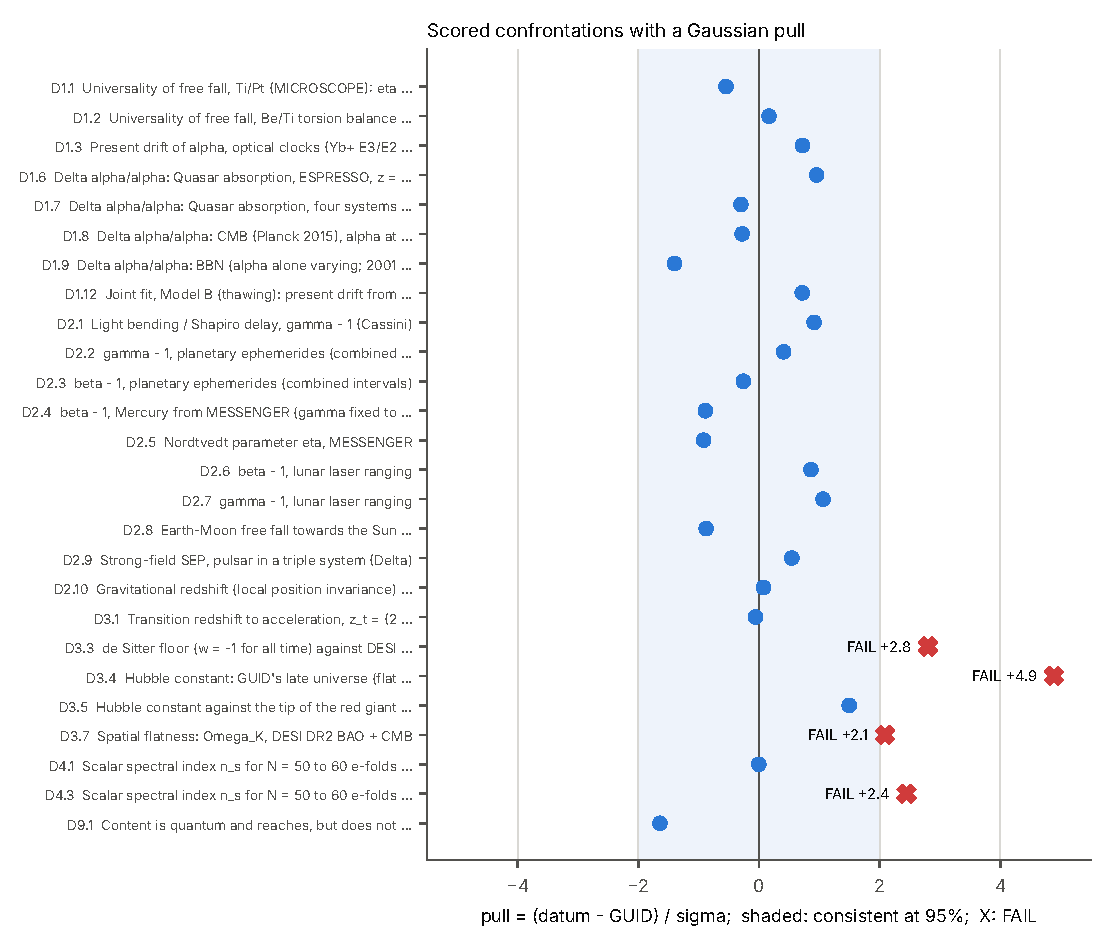
\includegraphics[width=0.74\linewidth]{data_pulls.pdf}
\caption{Pulls $p=(x-x_G)/\sigma$ of every scored confrontation with a Gaussian datum (Table~\ref{tab:data-master}; bounds and
qualitative rows are not shown). The shaded band is $|p|<1.96$, consistency at 95\%; crosses mark the four FAILs. What to look for: the
general-relativistic rows of D2 scatter within $1.1\sigma$; the FAILs are all cosmological (D3) or concern the spectral index (D4).}
\label{fig:data-pulls}
\end{figure}

\subsection{D1: the information scalar}\label{sec:data-alpha}

\paragraph{Model.} Hypothesis~4 adds to the content one scalar $\phi$ that sets the fine-structure constant (Section~\ref{sec:alpha}).
In units $\hbar=c=1$ with $\bar M_P^2=1/8\pi G$, the action of Part~I gives it the kinetic term $-\tfrac12\bar M_P^2(\partial\phi)^2$ and the
coupling $\lambda=\dd\ln\alpha/\dd\phi$ \tagH. A body whose mass has electrostatic share $f_A=E_{\rm C}/m_Ac^2$ has $\partial\ln m_A/\partial\phi
=\lambda f_A$, so the exchange of $\phi$ adds $2\lambda^2f_Af_B$ to the Newtonian force between two bodies, and two bodies falling towards
the Earth differ by $\eta=2\lambda^2f_\oplus(f_1-f_2)$ (Section~\ref{sec:fix}; Dvali and Zaldarriaga~\cite{dz}) \tagP. With the Coulomb
term $a_CZ(Z-1)/A^{1/3}$ of the semi-empirical mass formula, $f_{\rm Ti}=2.02\times10^{-3}$, $f_{\rm Pt}=4.05\times10^{-3}$,
$f_{\rm Be}=4.89\times10^{-4}$ and, for a coarse composition of the Earth, $f_\oplus=1.71\times10^{-3}$, so MICROSCOPE's
$\eta(\mathrm{Ti},\mathrm{Pt})=k\lambda^2$ with $k=-6.94\times10^{-6}$ \chk{data:D1.1}.

\paragraph{The coupling.} The likelihood is $\chi^2_{\rm EP}(\lambda)=\sum_i[(k_i\lambda^2-\eta_i)/\sigma_i]^2$ over MICROSCOPE~\cite{microscope}
(statistical and systematic errors in quadrature, $2.75\times10^{-15}$) and the E\"ot-Wash Be/Ti balance~\cite{schlamminger2008}, profiled with
$\lambda^2\ge0$. The best fit is $|\lambda|=1.47\times10^{-5}$, not significant, and the 95\% bound ($\Delta\chi^2=3.84$) is
\begin{equation}\label{eq:data-lambda}
|\lambda|<3.1\times10^{-5}\qquad(95\%\ \mathrm{CL})\quad\chk{data:D1.1},
\end{equation}
set by MICROSCOPE alone. The value $2\times10^{-5}$ used in earlier versions corresponds to $|\eta|<2.7\times10^{-15}$, a one-standard-deviation
bound.

\paragraph{Model A: the action as written.} Part~I's action has no potential for $\phi$. The scalar is then driven only by the
electromagnetic energy of matter, as in the theories of Bekenstein~\cite{bekenstein82} and of Sandvik, Barrow and Magueijo~\cite{bsbm}.
Dark matter, a gravitational remnant, carries none; baryons carry an electrostatic share $f_b>0$. For pressureless baryons with
$\partial\rho_b/\partial\phi=\lambda f_b\rho_b$, the field equation $\bar M_P^2\Box\phi=\partial\rho_b/\partial\phi$ in a flat
Friedmann universe reads, with $N=\ln a$ and $\phi'=\dd\phi/\dd N$,
\begin{equation}\label{eq:data-modelA}
\phi''+\Big(3+\frac{\dd\ln H}{\dd N}\Big)\phi'=-3\lambda f_b\,\Omega_b(N) ,
\end{equation}
where $\Omega_b(N)$ is the baryon share of the critical density at that time. In the matter era $\dd\ln H/\dd N=-3/2$ and the solution
approaches the attractor $\phi'=-2\lambda f_b\,\Omega_b/\Omega_m$, whatever the initial velocity (checked numerically, \chk{data:method}). Solving
\eqref{eq:data-modelA} through the present in flat $\Lambda$CDM (Planck 2018~\cite{planck18}) gives $\phi'_0=-0.141\,\lambda f_b$, so
\begin{equation}\label{eq:data-driftA}
\frac{\dot\alpha}{\alpha}\Big|_0=\lambda H_0\phi'_0=-9.70\times10^{-12}\,\lambda^2f_b\ \mathrm{yr}^{-1}\ \le0\qquad\chk{data:D1.3}.
\end{equation}
The sign follows from $\lambda^2\ge0$ and $f_b>0$: the scalar rolls towards lower matter energy, and with a positive electrostatic share that
lowers $\alpha$. GUID's forward statement, that $\alpha$ does not grow, is therefore \vd{derived} in Model A. Its size is not observable. The
helium Coulomb energy alone gives $f_b=6.0\times10^{-5}$; even with $f_b=10^{-3}$, taken as a generous upper value for the
electromagnetic self-energy of nucleons, and $|\lambda|$ at the bound~\eqref{eq:data-lambda}, the drift is $-9.6\times10^{-24}$ per year,
four orders of magnitude below the clocks, and $\Delta\alpha/\alpha=2.1\times10^{-12}$ at recombination \chk{data:D1.3}.

\paragraph{Model B: a slowly rolling scalar.} To ask what the data can say at all, we give the scalar a linear potential
$V=V_0-s\phi$ and make it the thawing dark energy: frozen by Hubble friction at early times, rolling late. For a canonical scalar
$\rho_\phi+p_\phi=\bar M_P^2\dot\phi^2$ holds exactly, so $\phi'^2=3\,\Omega_\phi(1+w)$ at every epoch. For small slopes the history has a
universal shape, and every $\alpha$ datum measures the present drift $d\equiv\dot\alpha/\alpha|_0$:
\begin{equation}\label{eq:data-G}
\frac{\Delta\alpha}{\alpha}(z)=-\frac{d}{H_0}\,G(z),\qquad G(z)=\int_{-\ln(1+z)}^{0}\frac{\phi'(N)}{\phi'(0)}\,\dd N ,
\end{equation}
with $G=0.118$ at Oklo ($z=0.137$, the 1.8\,Gyr implied by Damour and Dyson's quoted bound and rate~\cite{damour1996}), $0.435$ at
$z=1.15$, $0.514$ at $z=6.3$ and $0.516$ from recombination back, where the field is frozen; for $1+w_0=0.16$ these change by less than
2\% \chk{data:D1.12}. Each datum $i$ then gives $d_i=-H_0(\Delta\alpha/\alpha)_i/G(z_i)$, and Table~\ref{tab:data-alpha} and
Fig.~\ref{fig:data-alpha}a show what each allows. The clock value of Filzinger et al.~\cite{filzinger2023} includes the data of Lange et
al.~\cite{lange} and replaces it. The weighted mean is
\begin{equation}
d=(1.79\pm2.49)\times10^{-19}\ \mathrm{yr}^{-1},\qquad \chi^2=3.05\ \text{for 5 degrees of freedom},\qquad P(d<0)=0.24\qquad\chk{data:D1.12}.
\end{equation}

\begin{table}[tbp]
\centering\small
\caption{The present drift of $\alpha$ that each datum implies in Model B, Eq.~\eqref{eq:data-G} (one standard deviation).}
\label{tab:data-alpha}
\begin{tabular}{@{}lllll@{}}
\toprule
datum & $z$ & $G(z)$ & implied drift [$\mathrm{yr}^{-1}$] & source \\
\midrule
optical clocks & 0 & -- & $(1.8\pm2.5)\times10^{-19}$ & \cite{filzinger2023} \\
Oklo & 0.137 & 0.118 & $(0.0\pm3.3)\times10^{-18}$ & \cite{davis2015} \\
quasar, ESPRESSO & 1.15 & 0.435 & $(-2.1\pm2.2)\times10^{-16}$ & \cite{espresso} \\
quasars & 6.3 & 0.514 & $(2.9\pm9.7)\times10^{-15}$ & \cite{wilczynska2020} \\
CMB & 1100 & 0.516 & $(0.9\pm3.3)\times10^{-13}$ & \cite{hart2018} \\
BBN & $10^9$ & 0.516 & $(0.9\pm0.7)\times10^{-12}$ & \cite{avelino2001} \\
\midrule
joint & & & $(1.79\pm2.49)\times10^{-19}$ & \\
\bottomrule
\end{tabular}
\end{table}

\paragraph{What the data say about the sign.} Nothing. The clocks dominate the joint fit by an order of magnitude over Oklo and three over
the quasars; their central value is positive at $0.7\sigma$, and the 95\% interval $[-3.1,6.7]\times10^{-19}$ per year contains zero and both
signs. In Model B the drift and the coupling are separate parameters, linked only by the field speed, $d=\lambda H_0\phi'_0$, which the
dark energy's equation of state fixes. If the scalar were the field behind the evolving dark energy that DESI prefers, with $1+w_0=0.162$
(Section~\ref{sec:data-tensions}) and so $\phi'_0=0.577$, the clocks would demand $|\lambda|<1.7\times10^{-8}$, about two thousand times below the
free-fall bound; for $1+w_0=10^{-3}$, $|\lambda|<2.1\times10^{-7}$ \chk{data:D1.12}. Fig.~\ref{fig:data-alpha}b draws the allowed region.

\begin{figure}[tbp]
\centering
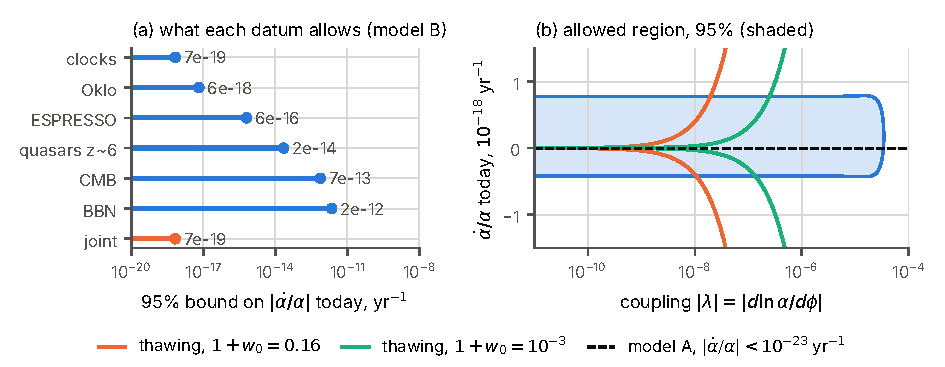
\includegraphics[width=\linewidth]{data_alpha_scalar.pdf}
\caption{The information scalar. (a) The 95\% bound on the present drift of $\alpha$ implied by each datum in Model B,
Eq.~\eqref{eq:data-G}, and by all together (data: Table~\ref{tab:data-alpha}). (b) The 95\% allowed region (shaded) in the plane of the coupling
$|\lambda|$ and the present drift, from free fall (MICROSCOPE, E\"ot-Wash) and the $\alpha$ data. Coloured curves: the drift a thawing dark
energy would impose, $d=\pm\lambda H_0\phi'_0$, for $1+w_0=0.16$ and $10^{-3}$; dashed: Model A, whose drift is below $10^{-23}$ per year.
What to look for: the region is a band around zero drift, symmetric in sign; a scalar that rolls with the dark energy must couple below
$10^{-8}$ to $10^{-7}$.}
\label{fig:data-alpha}
\end{figure}

\paragraph{Result.} Every $\alpha$ datum is consistent with GUID (D1.1 to D1.12). Free fall \vd{holds}; the coupling is bounded by
Eq.~\eqref{eq:data-lambda}; the negative drift is \vd{derived} for the action as written and \vd{untested}, since it is far below any
measurement; in a model where the drift could be seen, its sign is not predicted.

\subsection{D2: post-Newtonian gravity}\label{sec:data-ppn}

Minimal coupling (Section~\ref{sec:fix}) gives the post-Newtonian limit of general relativity: $\gamma=\beta=1$, no preferred-frame or
Nordtvedt effect, $\eta_N=4(\beta-1)-(\gamma-1)=0$~\cite{fienga2024} \tagP, the gravitational redshift of the lapse, and massless classical gravitational waves at $c$ with two tensor
polarisations (no graviton as a quantum of the frame). The twelve confrontations of Table~\ref{tab:data-master} all hold, with the
largest pull $1.06\sigma$ (lunar $\gamma$) and $\chi^2=5.63$ for 10 Gaussian pulls, $p=0.84$; the data partly overlap (Cassini radio data enter
the ephemerides), so that value is indicative \chk{data:D2}. The newest ephemeris combination gives $\beta-1=(-0.45\pm1.75)\times10^{-5}$ and
$\gamma-1=(0.55\pm1.35)\times10^{-5}$~\cite{fienga2024}; the pulsar in a triple system~\cite{voisin2020} tests the strong equivalence principle with a
neutron star. The final GWTC-3 tests bound the graviton mass by
$2.42\times10^{-23}\,\mathrm{eV}/c^2$ at 90\% credibility and find no non-tensor polarisation~\cite{ligo2025a}. The lunar errors of
Biskupek et al.\ are read as one standard deviation, which their paper does not state; that is the stricter reading. \emph{Verdict:}
\vd{holds}, and adds nothing general relativity does not predict.

\subsection{D3: the balanced state}\label{sec:data-cosmo}

GUID's late universe is flat $\Lambda$CDM settling into de Sitter expansion, $H\to H_\infty=\sqrt{\Omega_\Lambda}H_0$ (Section~\ref{sec:cosmo}).
Acceleration begins where $\ddot a=0$, at $z_t=(2\Omega_\Lambda/\Omega_m)^{1/3}-1$: $0.632\pm0.018$ for Planck's $\Omega_m=0.315\pm0.007$~\cite{planck18}
and $0.664\pm0.009$ for DESI DR2 with the CMB, $\Omega_m=0.3027\pm0.0036$~\cite{desi2} \chk{data:D3.1}. Two independent determinations of $z_t$
were found: $0.4\pm0.1$ from cosmic chronometers~\cite{moresco2016}, and $0.883\pm0.110$ from type Ia supernovae with $H(z)$~\cite{jesus2018}, the
mean of three parametrisations (0.806, 0.870, 0.973) with half their spread added as a systematic error. They pull against GUID by $-2.3\sigma$ and
$+2.2\sigma$ and disagree with each other by $3.2\sigma$, so at least one carries an unquoted systematic error. Combined with the scale factor
$S=3.25$ they give $0.62\pm0.24$, a pull of $-0.06\sigma$ \chk{data:D3.1}. A model-dependent analysis finds best fits between 0.61 and 0.82 for four
dark-energy models~\cite{dahiya2023}. The de Sitter rate is derived, not measured: $H_\infty=55.79\pm0.60$ (Planck) and $56.93\pm0.28\,
\mathrm{km\,s^{-1}Mpc^{-1}}$ (DESI with the CMB), $c/H_\infty=1.66\times10^{26}$\,m; it exists only if $w=-1$ \chk{data:D3.2}.

The direct test of the floor is the equation of state. DESI DR2 fits $w(a)=w_0+w_a(1-a)$ and finds, with the CMB, $w_0=-0.42\pm0.21$,
$w_a=-1.75\pm0.58$, a preference over $\Lambda$CDM of $3.1\sigma$; adding supernovae gives 2.8, 3.8 and $4.2\sigma$ for Pantheon+, Union3 and the
DES five-year sample~\cite{desi2}. A recalibration of the DES supernovae lowers its value to $3.2\sigma$, with $w_0=-0.803\pm0.054$, $w_a=-0.72\pm0.21$
and Bayesian odds of about 5:1~\cite{popovic2025}. We score the least significant combination, $2.8\sigma$: a FAIL at 95\% \chk{data:D3.3}. The
Hubble constant of the same model, $67.4\pm0.5\,\mathrm{km\,s^{-1}Mpc^{-1}}$, disagrees with the Cepheid ladder, $73.04\pm1.04$~\cite{riess2022},
by $4.9\sigma$, and agrees with the tip of the red giant branch, $70.39\pm1.94$~\cite{freedman2025}, at $1.5\sigma$ \chk{data:D3.4,D3.5}.
Inflation predicts $|\Omega_K|\lesssim10^{-5}$; Planck with BAO confirms flatness to 0.4\% at 95\%~\cite{planck2020x}, and DESI with the CMB finds
$\Omega_K=(2.3\pm1.1)\times10^{-3}$, $2.1\sigma$ from flat, while stating no significant preference for curvature~\cite{desi2} \chk{data:D3.6,D3.7}.
Section~\ref{sec:data-tensions} discusses the three FAILs.

\begin{figure}[tbp]
\centering
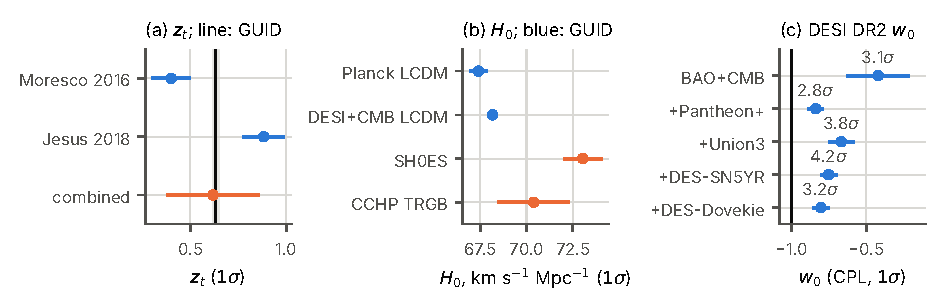
\includegraphics[width=\linewidth]{data_cosmology.pdf}
\caption{The balanced state against data (one standard deviation). (a) The transition redshift: GUID with Planck's $\Omega_m$ (line and
band), the two determinations~\cite{moresco2016,jesus2018} and their combination with the scale factor $S=3.25$. (b) $H_0$: the $\Lambda$CDM fits
that GUID inherits (Planck; DESI with the CMB) against the Cepheid ladder~\cite{riess2022} and the tip of the red giant branch~\cite{freedman2025}.
(c) $w_0$ of DESI DR2 for five data combinations~\cite{desi2,popovic2025}, with the quoted significance of the preference over $w=-1$ (line). What to
look for: GUID sits between the two $z_t$ values; it is far from SH0ES, close to the TRGB value; every DESI combination lies above $w=-1$.}
\label{fig:data-cosmo}
\end{figure}

\subsection{D4: inflation and the start}\label{sec:data-infl}

Part~I makes the start an inflation that ends in oscillons and names Starobinsky's $R^2$ inflation~\cite{starobinsky80}, with Higgs inflation as an
open alternative~\cite{bezrukov}. At leading order in $1/N$ both predict $n_s=1-2/N$ and $r=12/N^2$ for $N$ e-folds between the exit of the pivot
scale and the end of inflation, $n_s=0.960$ to $0.967$ and $r=0.0048$ to $0.0033$ for $N=50$ to $60$ \tagP. Against Planck
($n_s=0.9649\pm0.0042$~\cite{planck2020x}) the band holds, with pulls $+1.17$ to $-0.42\sigma$ and 95\% consistency for $46\le N\le74$. ACT DR6
moves $n_s$ up: $0.9709\pm0.0038$ with Planck (P-ACT; reported, not scored, as it overlaps both neighbours) needs $N\ge54.7$, and
$0.974\pm0.003$ with CMB lensing and DESI DR1 BAO (P-ACT-LB)~\cite{louis2025} needs $N\ge62.7$: for $N=60$ the pull is $+2.44\sigma$, a FAIL
\chk{data:D4.1,D4.3}. The ratio $r\le0.0048$ lies far below $r<0.036$~\cite{bk18} \chk{data:D4.4}; GUID itself allows the standard tensor spectrum,
generated within the start. Hypothesis~6$'$ puts the strong split before or during inflation. Had it come after, the Kibble--Preskill estimate,
one monopole per horizon at $T_c\sim10^{16}$\,GeV~\cite{preskill}, would give a flux of order $4\times10^2\,\mathrm{cm^{-2}s^{-1}sr^{-1}}$ at
$v=10^{-3}c$, $3\times10^{18}$ times MACRO's bound~\cite{macro}; inflation dilutes it to nothing \chk{data:D4.5} (scored once, as D8.2). The
ordering also needs reheating below the unification energy. Instantaneous reheating at the tensor bound would give at most $5.7\times10^{15}$\,GeV,
against $M_X\gtrsim4.8\times10^{15}$\,GeV from proton decay in the estimate of \chk{Q20}; the data allow either order, so this is a constraint on the
reheating model, not a test \chk{data:D4.6}.

\begin{figure}[tbp]
\centering
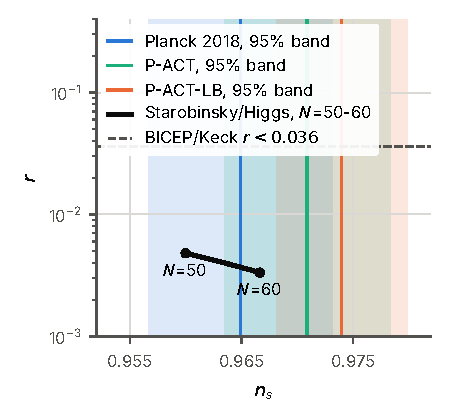
\includegraphics[width=0.58\linewidth]{data_inflation.pdf}
\caption{Starobinsky and Higgs inflation at leading order, $n_s=1-2/N$, $r=12/N^2$ for $N=50$ to $60$ (black), against the 95\% bands of $n_s$
from Planck 2018~\cite{planck2020x}, P-ACT and P-ACT-LB~\cite{louis2025}, and the BICEP/Keck bound $r<0.036$~\cite{bk18} (dashed). What to look for:
the line lies inside the Planck band, partly inside P-ACT and outside P-ACT-LB.}
\label{fig:data-infl}
\end{figure}

\subsection{D5: black holes}\label{sec:data-bh}

GUID's black holes are Kerr's (Section~\ref{sec:bh}): Christodoulou's mass formula~\cite{christodoulou} has no solution above $|a|=1$, the spin
energy is extracted in the ergosphere, and the area never shrinks classically. Matter that reaches the innermost stable circular orbit of a
thin disk radiates the binding energy $\epsilon(a)=1-E_{\rm isco}(a)$ (Bardeen, Press and Teukolsky~\cite{bpt}): $0.0377$ for a retrograde orbit
at $a=-1$, $0.0572$ at $a=0$ and $0.423$ as $a\to1$ \chk{data:D5}. The Soltan argument compares the light of all quasars with the mass in
black holes today. Its efficiencies are $0.04$ to $0.16$~\cite{marconi2004}, $0.075$ to $0.094$~\cite{shankar2009}, above $0.1$ for luminous
quasars~\cite{yu2002}, and a mean of $0.089$ for individual thin-disk fits~\cite{davis2011}. All lie below the Kerr maximum. Read on the Kerr
curve they imply typical spins of $0.40$ to $0.62$, above $0.67$ for luminous quasars, and $0.58$ at the mean of Davis and Laor
(Fig.~\ref{fig:data-kerr}a). The curve bounds the efficiency only from above, since radiatively inefficient flows can fall below $5.7\%$.
All 61 measured spins in the compilation of Reynolds~\cite{reynolds2021}, 36 supermassive (X-ray reflection) and 25 stellar (reflection and
continuum fitting), lie in $[-1,1]$ at 90\%, most supermassive ones above $0.9$ (Fig.~\ref{fig:data-kerr}b). The test is weak, since the
spectral models are Kerr models capped at $a=0.998$. The ringdown of GW150914 shows an area increase with probability 0.97 (0.95 without
overtones)~\cite{isi2021}, and that of GW250114 shows it ``to high credibility''~\cite{ligo2025b} \chk{data:D5.6,D5.7}. Hawking radiation of a
solar-mass hole, at $6.2\times10^{-8}$\,K, is unobservable and unobserved. \emph{Verdict:} \vd{holds}, with general relativity.

\begin{figure}[tbp]
\centering
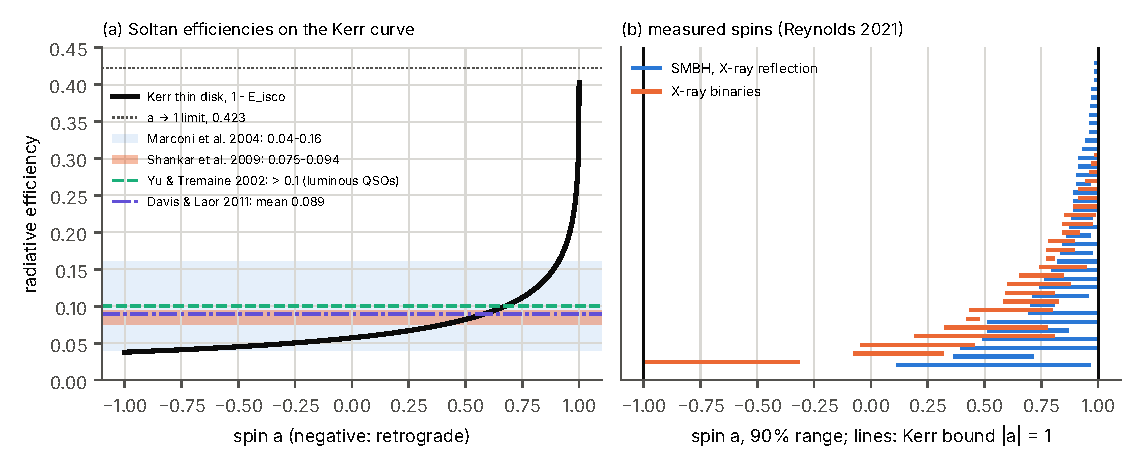
\includegraphics[width=\linewidth]{data_kerr.pdf}
\caption{Black holes. (a) The thin-disk efficiency of Kerr accretion against the spin (black), with the Soltan efficiencies of
Refs.~\cite{marconi2004,shankar2009,yu2002,davis2011}; where a band meets the curve it reads off the typical spin. (b) The 90\% ranges of 36
supermassive and 25 stellar spins~\cite{reynolds2021}, sorted; vertical lines: the Kerr bound. What to look for: every efficiency is below the
$a\to1$ limit, and no spin range leaves $[-1,1]$.}
\label{fig:data-kerr}
\end{figure}

\subsection{D6: Bridge B against the largest superpositions}\label{sec:data-bridgeB}

Bridge B (Section~\ref{sec:bridges}) holds the decoherence-diffusion trade-off at equality with a record at Planck strength and lands on the
Di\'osi--Penrose rate~\cite{diosi87,penrose96} $\Gamma=E_\Delta/\hbar$, with
\begin{equation}\label{eq:data-EDelta}
E_\Delta=\frac G2\iint\frac{[\rho_1(\mathbf x)-\rho_2(\mathbf x)][\rho_1(\mathbf y)-\rho_2(\mathbf y)]}{|\mathbf x-\mathbf y|}\,\dd^3x\,\dd^3y
\end{equation}
for a mass in a superposition of densities $\rho_1$ and $\rho_2$; Part~I uses its order of magnitude $\Gamma=GM^2/\hbar R$. For a uniform sphere
displaced by $d=xR$, Eq.~\eqref{eq:data-EDelta} gives $E_\Delta=(GM^2/R)(x^2/2-3x^3/16+x^5/160)$ for $x<2$ and $(GM^2/R)(6/5-1/x)$ for $x\ge2$; for a
mass smeared as a Gaussian of width $s$, $E_\Delta=GM^2[1/(\sqrt\pi s)-\mathrm{erf}(d/2s)/d]$. Both closed forms agree with Fourier quadrature
\chk{data:method}. For each of the largest existing superpositions we take the larger of $GM^2/\hbar R$ and the full $E_\Delta/\hbar$. The full
value is the bulk sphere plus every nucleus smeared over the smallest allowed width $R_0=0.54\times10^{-10}$\,m, since a larger $R_0$ lowers
the rate; an atom is its nucleus smeared over $R_0$. The predicted loss of coherence during the observed coherence time $\tau$ is $\Gamma\tau$
(Table~\ref{tab:data-bridgeB}).

\begin{table}[tbp]
\centering\small
\caption{Bridge B against the largest existing superpositions. $\Gamma$: the larger of the two rate estimates (see text); margin: $1/\Gamma\tau$.
Molecule radius estimated from mass and a density of 1300\,kg/m$^3$; cluster diameter 8\,nm as stated; separation for the clusters: the stated
lower bound of ten diameters.}
\label{tab:data-bridgeB}
\begin{tabular}{@{}llllll@{}}
\toprule
experiment & mass [kg] & separation & $\tau$ [s] & $\Gamma$ [s$^{-1}$] & margin \\
\midrule
oligoporphyrins, 28\,kDa~\cite{fein2019} & $4.6\times10^{-23}$ & 266\,nm & $7\times10^{-3}$ & $8.1\times10^{-13}$ & $2\times10^{14}$ \\
Na clusters, 197\,kDa~\cite{pedalino2025} & $3.3\times10^{-22}$ & 80\,nm & $1.2\times10^{-2}$ & $2.0\times10^{-11}$ & $4\times10^{12}$ \\
Rb atoms~\cite{kovachy2015} & $1.4\times10^{-25}$ & 54\,cm & 1 & $2.4\times10^{-16}$ & $4\times10^{15}$ \\
Cs atoms~\cite{xu2019} & $2.2\times10^{-25}$ & 3.9\,$\mu$m & 20 & $5.7\times10^{-16}$ & $9\times10^{13}$ \\
\bottomrule
\end{tabular}
\end{table}

All four pass with margins of $4\times10^{12}$ to $4\times10^{15}$ \chk{data:D6.1-D6.4}: existing interferometry does not reach Bridge B. The
smearing length is free in Bridge B. The absence of spontaneous radiation in an underground germanium detector requires $R_0>0.54\times10^{-10}$\,m
with probability 0.95~\cite{donadi}. That excludes Penrose's parameter-free choice, the nuclear wave-function size, $5\times10^{-12}$\,m for
germanium. Figurato et al.\ summarise current bounds as $R_0\gtrsim4\times10^{-10}$\,m~\cite{figurato}. Bridge B therefore needs
$R_0\ge4\times10^{-10}$\,m; at that smearing the bulk term still dominates the $10^{-14}$\,kg sphere by more than a factor $10^3$ \chk{data:D6.5,D6.6,data:method}.
The diffusion coefficient of the Di\'osi--Penrose kernel, $l_P^2D_2=m_P^2/c=1.6\times10^{-24}\,\mathrm{kg^2\,s/m}$, lies inside the window
$10^{-40}$ to $10^{-9}$ that torsion balances and molecule interferometry leave~\cite{osswd}, while the discrete version, $m_Pt_P=1.2\times10^{-51}$\,kg\,s,
lies below its window $10^{-25}$ to $10^{-1}$ and is excluded, as Part~I states \chk{data:D6.8,D6.9}.

\paragraph{The smallest decisive experiment.} The Di\'osi--Penrose coherence time of a uniform sphere separated by more than its size is
$\tau_{\rm DP}=\hbar R/(\tfrac65GM^2)\propto M^{-5/3}$. A silica sphere reaches $\tau_{\rm DP}=10$\,ms at $1.2\times10^{-14}$\,kg, 1\,s at
$7.6\times10^{-16}$\,kg and 100\,s at $4.8\times10^{-17}$\,kg \chk{data:D6}. The first experiment to see Bridge B is a centre-of-mass
superposition of such a particle, separated by more than its diameter and held that long. That is five to eight orders of magnitude in mass
beyond the heaviest superposition so far, $3.3\times10^{-22}$\,kg~\cite{pedalino2025} (Fig.~\ref{fig:data-bridgeB}). The diamond microsphere of the
Bose et al.\ proposal~\cite{bose} ($10^{-14}$\,kg, radius $0.88\,\mu$m) decoheres in 13.9\,ms by $GM^2/\hbar R$ and in 11.6\,ms by
Eq.~\eqref{eq:data-EDelta} at 250\,$\mu$m separation, long before its 8 to 25\,s entangling time; Section~\ref{sec:bmv} treats that experiment.
\emph{Verdict:} Bridge B is consistent with every superposition made, but no superposition made tests it: \vd{live}, \vd{untested}.

\begin{figure}[tbp]
\centering
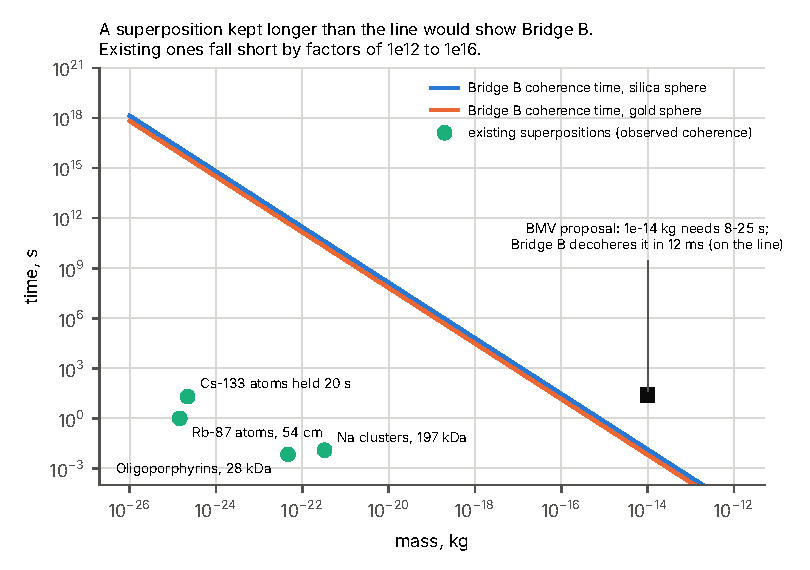
\includegraphics[width=0.66\linewidth]{data_bridgeB.pdf}
\caption{Bridge B's coherence time $\hbar R/(\tfrac65GM^2)$ for silica and gold spheres (lines) against the observed coherence of the largest
superpositions (dots: Refs.~\cite{fein2019,pedalino2025,kovachy2015,xu2019}) and the Bose et al.\ proposal~\cite{bose} (square: the time it needs,
8 to 25\,s). A superposition kept above the line would show Bridge B's decoherence. What to look for: existing experiments fall short by twelve
to sixteen orders of magnitude; the proposal lies above the line, so Bridge B decoheres it in about 12\,ms.}
\label{fig:data-bridgeB}
\end{figure}

\subsection{D7: contained remnants}\label{sec:data-pbh}

The contained route makes dark matter of primordial black holes from the start in the window $10^{14}$ to $10^{19}$\,kg
(Section~\ref{sec:darkmatter}). For a monochromatic mass function, Gorton and Green find the window between about $10^{17}$ and $10^{22}$\,g open for
all of the dark matter; it narrows for extended mass functions~\cite{gortongreen}. Its light edge is set by the products of Hawking evaporation:
INTEGRAL/SPI gamma rays and the Voyager~1 positron and electron flux exclude all of the dark matter below about $10^{17}$\,g. Its heavy edge is
set by Subaru-HSC microlensing of M31, ineffective below about $10^{22}$\,g by wave optics. The Hawking temperatures at the edges are
$1.2\times10^9$\,K ($k_BT=0.11$\,MeV) and $1.2\times10^4$\,K \chk{data:D7.3}. The mass that has evaporated within 13.8\,Gyr,
$1.7\times10^{11}$\,kg by the Stefan--Boltzmann estimate, agrees within a factor of ten with the ``about $10^{15}$\,g'' of Carr et
al.~\cite{carr2021} \chk{data:D7.2}. \emph{Verdict:} \vd{live}. The window is open, and the prediction that its light edge glows is exactly
what bounds it.

\subsection{D8: the electroweak and strong splits}\label{sec:data-splits}

Hypothesis~6$'$ allows a unification before the start. Its heavy gauge bosons would still let protons decay, with $\tau\sim M_X^4/(\alpha_G^2m_p^5)$,
$4.6\times10^{35}$\,yr for $M_X=10^{16}$\,GeV and $\alpha_G=1/40$, above Super-Kamiokande's $2.4\times10^{34}$\,yr~\cite{superk};
Hyper-Kamiokande~\cite{hyperk} is the live test \chk{data:D8.1}. Relic monopoles are absent, as MACRO's flux bound requires~\cite{macro}
\chk{data:D8.2}. At the electroweak split the photon emerges with $e=g\sin\theta_W$, and the W and Z take their masses from the vacuum
$v=(\sqrt2G_F)^{-1/2}=246.22$\,GeV (from the muon lifetime~\cite{mulan2013}) \tagP. Part~I claims agreement within half a per cent at tree level.
From $1/\hat\alpha(M_Z)=127.950\pm0.017$~\cite{erler2017}, $\sin^2\hat\theta_W(M_Z)=0.23129\pm0.00004$~\cite{navas2024} and $G_F$, $m_W=(\pi\hat\alpha/
\sqrt2G_F\sin^2\hat\theta_W)^{1/2}=80.22$\,GeV is $0.18\%$ below the world average $80.369\pm0.013$\,GeV (without CDF)~\cite{lhctev2024}. Likewise
$m_Z=m_W/\cos\hat\theta_W=91.50$\,GeV is $0.34\%$ above $91.1880\pm0.0020$\,GeV~\cite{navas2024} \chk{data:D8.3,D8.4}. Tree level is scheme
dependent: $m_Z\cos\hat\theta_W=79.95$\,GeV, and the on-shell route from $\alpha(0)$, $G_F$ and $m_Z$ gives $80.94$\,GeV; the measured value lies
inside that $\pm0.6\%$ spread, and only the loop-level Standard Model reaches the experimental precision. The coupling is born near $1/128$,
$1/\hat\alpha(M_Z)=127.95$, and runs to $1/137.035999177(21)$~\cite{codata2022} \chk{data:D8.5}. A Higgs mass of $125.11\pm0.11$\,GeV~\cite{atlas2023}
lies far above the end point of the first-order line, between 70 and 95\,GeV~\cite{kajantie1996}. The split is therefore the smooth crossover
at $T_c=159.5\pm1.5$\,GeV found on the lattice~\cite{donofrio} \chk{data:D8.6}. \emph{Verdict:} \vd{holds}; all of it is the Standard Model's.

\subsection{D9: the rest}\label{sec:data-rest}

The content is quantum, so the CHSH combination reaches but does not exceed Tsirelson's bound $2\sqrt2$, while the gates give 2
(Section~\ref{sec:holo}). The most precise value, $S=2.82759\pm0.00051$~\cite{poh2015}, lies $1.64\sigma$ below the bound. The loophole-free
$S=2.42\pm0.20$~\cite{hensen2015} lies inside $(2,2\sqrt2]$ \chk{data:D9.1,D9.2}. The known neutrinos are not the remnant: DESI DR2 with the CMB bounds
$\sum m_\nu<0.064$\,eV (95\%), below 0.57\% of the dark matter density~\cite{desi2}, and KATRIN's $m_\nu<0.45$\,eV (90\%) leaves at most 12\%
in the laboratory~\cite{katrin2025} \chk{data:D9.3,D9.4}. The radiated remnant, the nanohertz background, has $\Omega_{\rm gw}\le1.3\times10^{-8}$ at
1/yr (upper end of the 90\% range of $h_c$~\cite{nanograv}) and is radiation, not dark matter \chk{data:D9.5}. Gravity weighs all energy
(Hypothesis~1$'$). A gravity that weighed only the Higgs-given share would make titanium and platinum fall apart at $\eta\sim10^{-3}$, which
MICROSCOPE excludes by $4\times10^{11}\sigma$ \chk{data:D9.6}.

\subsection{The four inherited tensions}\label{sec:data-tensions}

The four FAILs are real, and each is a tension of the established account that GUID adopts unchanged. GUID adds nothing that moves it.
\begin{enumerate}[nosep,leftmargin=*]
\item \emph{Evolving dark energy (D3.3).} The de Sitter floor needs $w=-1$ at all times. DESI DR2 prefers $w_0>-1$ with $w_a<0$ at 2.8 to $4.2\sigma$,
depending on the supernova sample, and $3.1\sigma$ without supernovae~\cite{desi2}. No combination reaches $5\sigma$. The DES recalibration
lowers its own value from $4.2\sigma$ to $3.2\sigma$, at odds of about 5:1~\cite{popovic2025}. In the parametrisation used, $w$ crosses $-1$ in the
past, which no single canonical scalar can do. If the preference holds, the end is not de Sitter, and the reading of the balanced state as a
de Sitter future (Section~\ref{sec:cosmo}) must be redone. An information scalar that rolled with that dark energy would also have to couple
below $1.7\times10^{-8}$ (Section~\ref{sec:data-alpha}).
\item \emph{The Hubble constant (D3.4).} The CMB-calibrated $\Lambda$CDM value lies $4.9\sigma$ from the Cepheid ladder and $1.5\sigma$ from the
tip of the red giant branch. The disagreement between the two local methods is part of the open question; GUID offers no resolution.
\item \emph{Curvature (D3.7).} DESI with the CMB finds $\Omega_K$ $2.1\sigma$ from zero; DESI itself reports no significant preference, and Planck
with BAO finds flatness to 0.4\%. With 58 scored rows, about three FAILs at 95\% are expected by chance.
\item \emph{The spectral index (D4.3).} At leading order, the plateau inflation Part~I names needs $N\ge63$ e-folds to meet ACT DR6 with lensing and
BAO, and $N\ge55$ to meet P-ACT, while Planck alone is satisfied for $N=50$ to 60. The shift comes partly from the BAO in the combination, which
also drives D3.3. How many e-folds belong to the pivot scale depends on the reheating history, so the gap of a few e-folds constrains
reheating as much as the potential. The model is in tension; GUID's start, which requires inflation but not this potential, is not.
\end{enumerate}

\subsection{No data yet}\label{sec:data-nodata}

The predictions that would tell GUID apart are not reached by any measurement:
gravitationally mediated entanglement, where GUID predicts $\mathcal N=0$~\cite{bose,mv}, and with Bridge B decoherence first (Section~\ref{sec:bmv});
the LOCC inequality of Lami, Pedernales and Plenio~\cite{lpp}, predicted to hold;
the decoherence-diffusion trade-off at equality, of which only the window of D6.8 is known;
Bridge B's own decoherence, which needs the masses of Section~\ref{sec:data-bridgeB};
single-graviton clicks, which do not discriminate;
primordial tensor modes, for which only the bound $r<0.036$ exists;
the Hawking glow at the light edge of the black-hole window, for which only bounds exist;
the return of information from evaporating holes;
proton decay;
and the sign of the drift of $\alpha$.

\paragraph{Choices made after seeing the data.} The two determinations of $z_t$ were combined with the scale factor after they were seen to
disagree with each other, and the three parametrisations of one paper were merged with their spread as a systematic error. The DESI test is
scored on the least significant combination. Of the three spectral-index data sets, Planck and P-ACT-LB are scored and P-ACT, which overlaps
both, is reported. The lunar laser-ranging errors are read as one standard deviation. The Kerr test uses the upper end of each efficiency
range. The evaporation mass of D7.2 is scored with a tolerance of a factor of ten. The Bridge B test counts a run as consistent below
$\Gamma\tau=0.1$. The monopole datum is scored once (D8.2), not twice. Model inputs that are not data were fixed as follows: $f_b=10^{-3}$ as an
upper value, the Oklo time of 1.8\,Gyr, the molecule density of 1300\,kg/m$^3$ and the cluster separation at its stated lower bound. No verdict
depends on any of these choices except that of D3.1, where scoring either $z_t$ determination alone would give a FAIL in one direction or
the other.

\paragraph{Caveats.} Several values were read through a web search because the journal or data-group page could not be opened. These are
Cassini's $\gamma$, MESSENGER's $\eta_N$, the PDG values of $m_Z$ and $\sin^2\hat\theta_W$, the 2017 PDG value of $\hat\alpha(M_Z)$, the CODATA value
of $\alpha$, the interferometer parameters of Fein et al., and the species and separations of Refs.~\cite{kovachy2015,xu2019}. The DESI
significances are the collaboration's conversions of $\Delta\chi^2$ for two extra parameters; the Model B mapping of $w_0$ to the field speed
uses the present-day value, which is exact, but the CPL fit is not a thawing fit. The nucleosynthesis datum uses 2001 abundances; more recent
analyses that vary all couplings together~\cite{martins2021} reach parts per million, but do not apply to a scalar that sets only $\alpha$. The
spins are measured with Kerr models, and the GW250114 statement is qualitative. The paper does not quote an area value or a significance
in standard deviations.

All numbers in this section come from \texttt{docs/simulation/predictions\_vs\_data.py}: 72 rows, 54 of 58 scored confrontations consistent
and 6 of 6 method checks, about four seconds on one core.

\paragraph{Verdict.} Of the 58 confrontations of GUID with current data that this section scores, 54 hold at 95\%. The four that do not are
tensions of $\Lambda$CDM and of plateau inflation that GUID inherits unchanged: evolving dark energy, the Hubble constant, a $2\sigma$
curvature and the spectral index. Free fall, the post-Newtonian parameters, Kerr black holes, the electroweak masses and the cosmological
bounds hold, but they hold for general relativity, $\Lambda$CDM and the Standard Model alike. The information scalar's negative drift is
derived and too small to measure. Bridge B lies five to eight orders of magnitude in mass beyond the largest superpositions made. No existing
datum can tell GUID apart; the experiments of Section~\ref{sec:exp} can.
